\documentclass[11pt]{article}
\usepackage[margin=1in]{geometry}
\usepackage[T1]{fontenc}
\usepackage{lmodern,amsmath,amssymb,booktabs,array,graphicx,longtable}
\usepackage[numbers,sort&compress]{natbib}
\usepackage{microtype,setspace,etoolbox}
\usepackage{caption}
\captionsetup[table]{font=small,skip=6pt}
% Keep table text at a fixed 9 pt; never enlarge a table to fill the line.
\newcommand{\tabletextstyle}{\footnotesize\setstretch{1.05}\setlength{\tabcolsep}{4pt}}
\AtBeginEnvironment{tabular}{\tabletextstyle}
\AtBeginEnvironment{longtable}{\tabletextstyle}
\usepackage[hidelinks]{hyperref}
\hypersetup{pdfauthor={},pdftitle={SimTIO: A Simulation-Grounded Multi-Agent LLM Framework for Compositional Traffic Intervention Optimization}}
\setstretch{1.15}
\setlength{\emergencystretch}{3em}
\renewcommand{\topfraction}{0.95}
\renewcommand{\bottomfraction}{0.85}
\renewcommand{\textfraction}{0.05}
\renewcommand{\floatpagefraction}{0.85}
\setcounter{topnumber}{4}
\setcounter{totalnumber}{6}
\newcommand{\WideLLMTop}{11.53}
\newcommand{\WideRuleTop}{12.10}
\newcommand{\WideRandomTop}{14.81}
\newcommand{\StrictLLMTop}{8.50}
\newcommand{\StrictRuleTop}{9.36}
\newcommand{\StrictRandomTop}{9.55}

\title{SimTIO: A Simulation-Grounded Multi-Agent LLM Framework for Compositional Traffic Intervention Optimization}
\author{}
\date{}
\begin{document}
\maketitle
\begin{abstract}
Traffic interventions can relieve local bottlenecks while transferring delay elsewhere. SimTIO is a simulation-grounded framework in which role-specific large language models (LLMs) select validated mutations and a constrained simulation rule determines the retained plan. The framework supports intervention composition and continued refinement using measured joint feedback. We evaluate five network extracts with three synthetic-demand seeds and 2,400 passenger trips per case. A frozen-input comparison holds initial candidates, parents, legal mutation catalogs, simulation seeds, and bundle rules constant while varying the selector. Its mean Top-10 time-loss reductions are 8.50\%, 9.36\%, and 9.55\% for LLM, rule-based, and random selection. A wider adaptive search yields 11.53\%, 12.10\%, and 14.81\%, respectively, with feasible plans in 13 of 15 cases for each method. Neither comparison establishes an LLM advantage. Five repeated LLM and random searches per fixed-demand case reveal substantial outcome variation in some networks. Additional tests at 1,200 and 3,600 trips change relative method performance; the highest-demand Manhattan cases include substantial teleport recovery and require qualification as simulation stress tests. Threshold reselection and full-network edge diagnostics show that aggregate feasibility can coexist with concentrated remote deterioration. The contribution is an auditable framework for constrained scenario screening and a controlled assessment of selector limitations. These uncalibrated passenger-demand experiments do not establish real-city traffic improvements or multimodal effectiveness.
\end{abstract}
\noindent\textbf{Keywords:} Traffic simulation; Large language models; Intervention composition; Constrained search; Synthetic demand; Spatial spillover

\section{Introduction}
Microscopic traffic simulation supports intervention comparison before implementation. Turning a bottleneck diagnosis into an executable scenario nevertheless requires selecting control targets, editing interdependent network and route files, and checking effects beyond the target roads. An intervention can be locally attractive yet violate throughput or network-delay requirements. Proposal generation and evidence for accepting a proposal should therefore remain distinct.

LLMs offer a common interface to heterogeneous intervention families. Their contribution, however, cannot be inferred from the performance of a pipeline that also contains grounded initialization, domain-specific catalogs, validators, feedback, and a final rejection rule. Giving an LLM three initial proposals followed by two refinements, while giving a baseline five independent proposals, confounds selector policy with search structure even when simulation caps match.

SimTIO organizes signal, network, and routing specialists around executable intervention catalogs and measured SUMO feedback. Compatible interventions can be composed, simulated jointly, and retained as parents for further conditional refinement. An explicit acceptance rule evaluates fixed baseline bottlenecks, neighboring spillover, network mean delay, demand completion, and teleports. The baseline remains available as a no-operation decision. Here, multi-agent denotes role-specific specialist calls and tool ownership; superiority over a centralized agent is not established.

Our contributions are a reproducible procedure for heterogeneous intervention screening, a frozen-input selector comparison that addresses search-structure confounding, and an evaluation of sampling, demand, threshold, and spatial limitations. We distinguish that controlled comparison from the full adaptive search, whose later catalogs can diverge following earlier choices. The results do not support a general LLM advantage. They identify which parts of the procedure are auditable and which performance claims remain unsupported.

City names identify network extracts, not calibrated traffic-management applications. Equal synthetic trip counts neither equalize saturation nor reproduce observed OD patterns. The present evidence concerns passenger vehicles and offline scenario screening across operational and planning horizons.

\section{Related work}
Simulation-based transportation optimization predates LLM-assisted search. Osorio and Bierlaire combine microscopic simulation with an analytical queueing model in a metamodel-based optimization procedure, while Osorio and Chong extend this approach to large-scale constrained signal optimization under limited computational budgets~\cite{osorio2013simulation,osorio2015large}. These studies establish relevant alternatives for allocating costly simulator evaluations. SimTIO instead searches discrete, heterogeneous scenario edits through finite catalogs. Our selector comparison does not benchmark against these metamodel methods and therefore does not establish an advantage over conventional simulation-based optimization.

Execution-grounded LLM optimization uses external evaluation to distinguish plausible proposals from successful ones. OPRO conditions proposals on previous solution--score pairs, Self-Refine uses iterative feedback, and FunSearch couples generated programs with deterministic evaluation~\cite{yang2024opro,madaan2023selfrefine,romera2024funsearch}. Evolution of Heuristics and ReEvo further organize iterative heuristic development~\cite{liu2024eoh,ye2024reevo}. These approaches motivate separating language generation from execution and measurement. SimTIO's search objects are structured interventions rather than arbitrary executable programs.

Agent architectures provide complementary mechanisms for connecting language models to external environments. ReAct interleaves reasoning and actions with observations, and Reflexion retains linguistic feedback to inform later attempts~\cite{yao2023react,shinn2023reflexion}. AutoGen organizes applications through configurable agent conversations, within a broader literature on autonomous-agent construction and evaluation~\cite{wu2024autogen,wang2024agentsurvey}. AgentBench documents limitations in long-horizon decision-making and instruction following across interactive tasks~\cite{liu2024agentbench}. These findings motivate evaluating executed outcomes and failure modes rather than treating a multi-agent architecture as evidence of optimization ability. SimTIO uses role-specific catalog selection and simulator-based acceptance; it does not evaluate these general-purpose agent frameworks as competing implementations.

Traffic control includes established feedback policies such as max-pressure control, whose throughput properties are derived under explicit queueing assumptions~\cite{varaiya2013maxpressure}, and learned policies such as PressLight and CoLight~\cite{wei2019presslight,wei2019colight}. LLM-based work includes structured phase selection and cooperative signal control~\cite{lai2025llmlight,yuan2026collmlight}. Other systems automate traffic-simulation workflows~\cite{anonymous2024,anonymous2026} or provide traffic-simulation agents~\cite{du2025trafficsimagent}. Our evaluation concerns offline selection among a limited number of scenario modifications, rather than a policy that acts at every signal cycle. Interaction between signal settings, route assignment, and network design motivates joint evaluation of intervention pairs~\cite{meneguzzer1997combined,yang1998networkdesign}. The classical traffic-planning paradox further shows that adding network capacity can increase equilibrium travel times~\cite{braess2005paradox}. This motivates measuring whole-network consequences; our experiments do not identify a Braess paradox or assume equilibrium assignment.

Application validity also depends on the simulation inputs and calibration. Hollander and Liu discuss parameter calibration, goodness-of-fit, and repeated runs, while the FHWA microsimulation guidelines connect observed conditions, calibration, and alternatives analysis~\cite{hollander2008calibration,wunderlich2019toolbox}. These requirements distinguish a reproducible algorithmic test from a validated transport application. Varying synthetic demand or model sampling can reveal conditional sensitivity, but it does not establish agreement with observed traffic.

\section{Methodology}\label{sec:methods}
Figure~\ref{fig:framework} presents the current adaptive protocol: baseline diagnosis, shared grounded initialization, catalog-based specialist refinement, compatible composition, continued joint feedback, and constrained selection. Initialization is program-generated; the LLM selects legal mutations of measured parents. A jointly simulated plan can become a parent for further conditional modification with one component held fixed, as specified in Section~\ref{sec:search}. The smaller frozen-input selector comparison is defined separately in Section~\ref{sec:matched}.

\begin{figure}[htbp]\centering
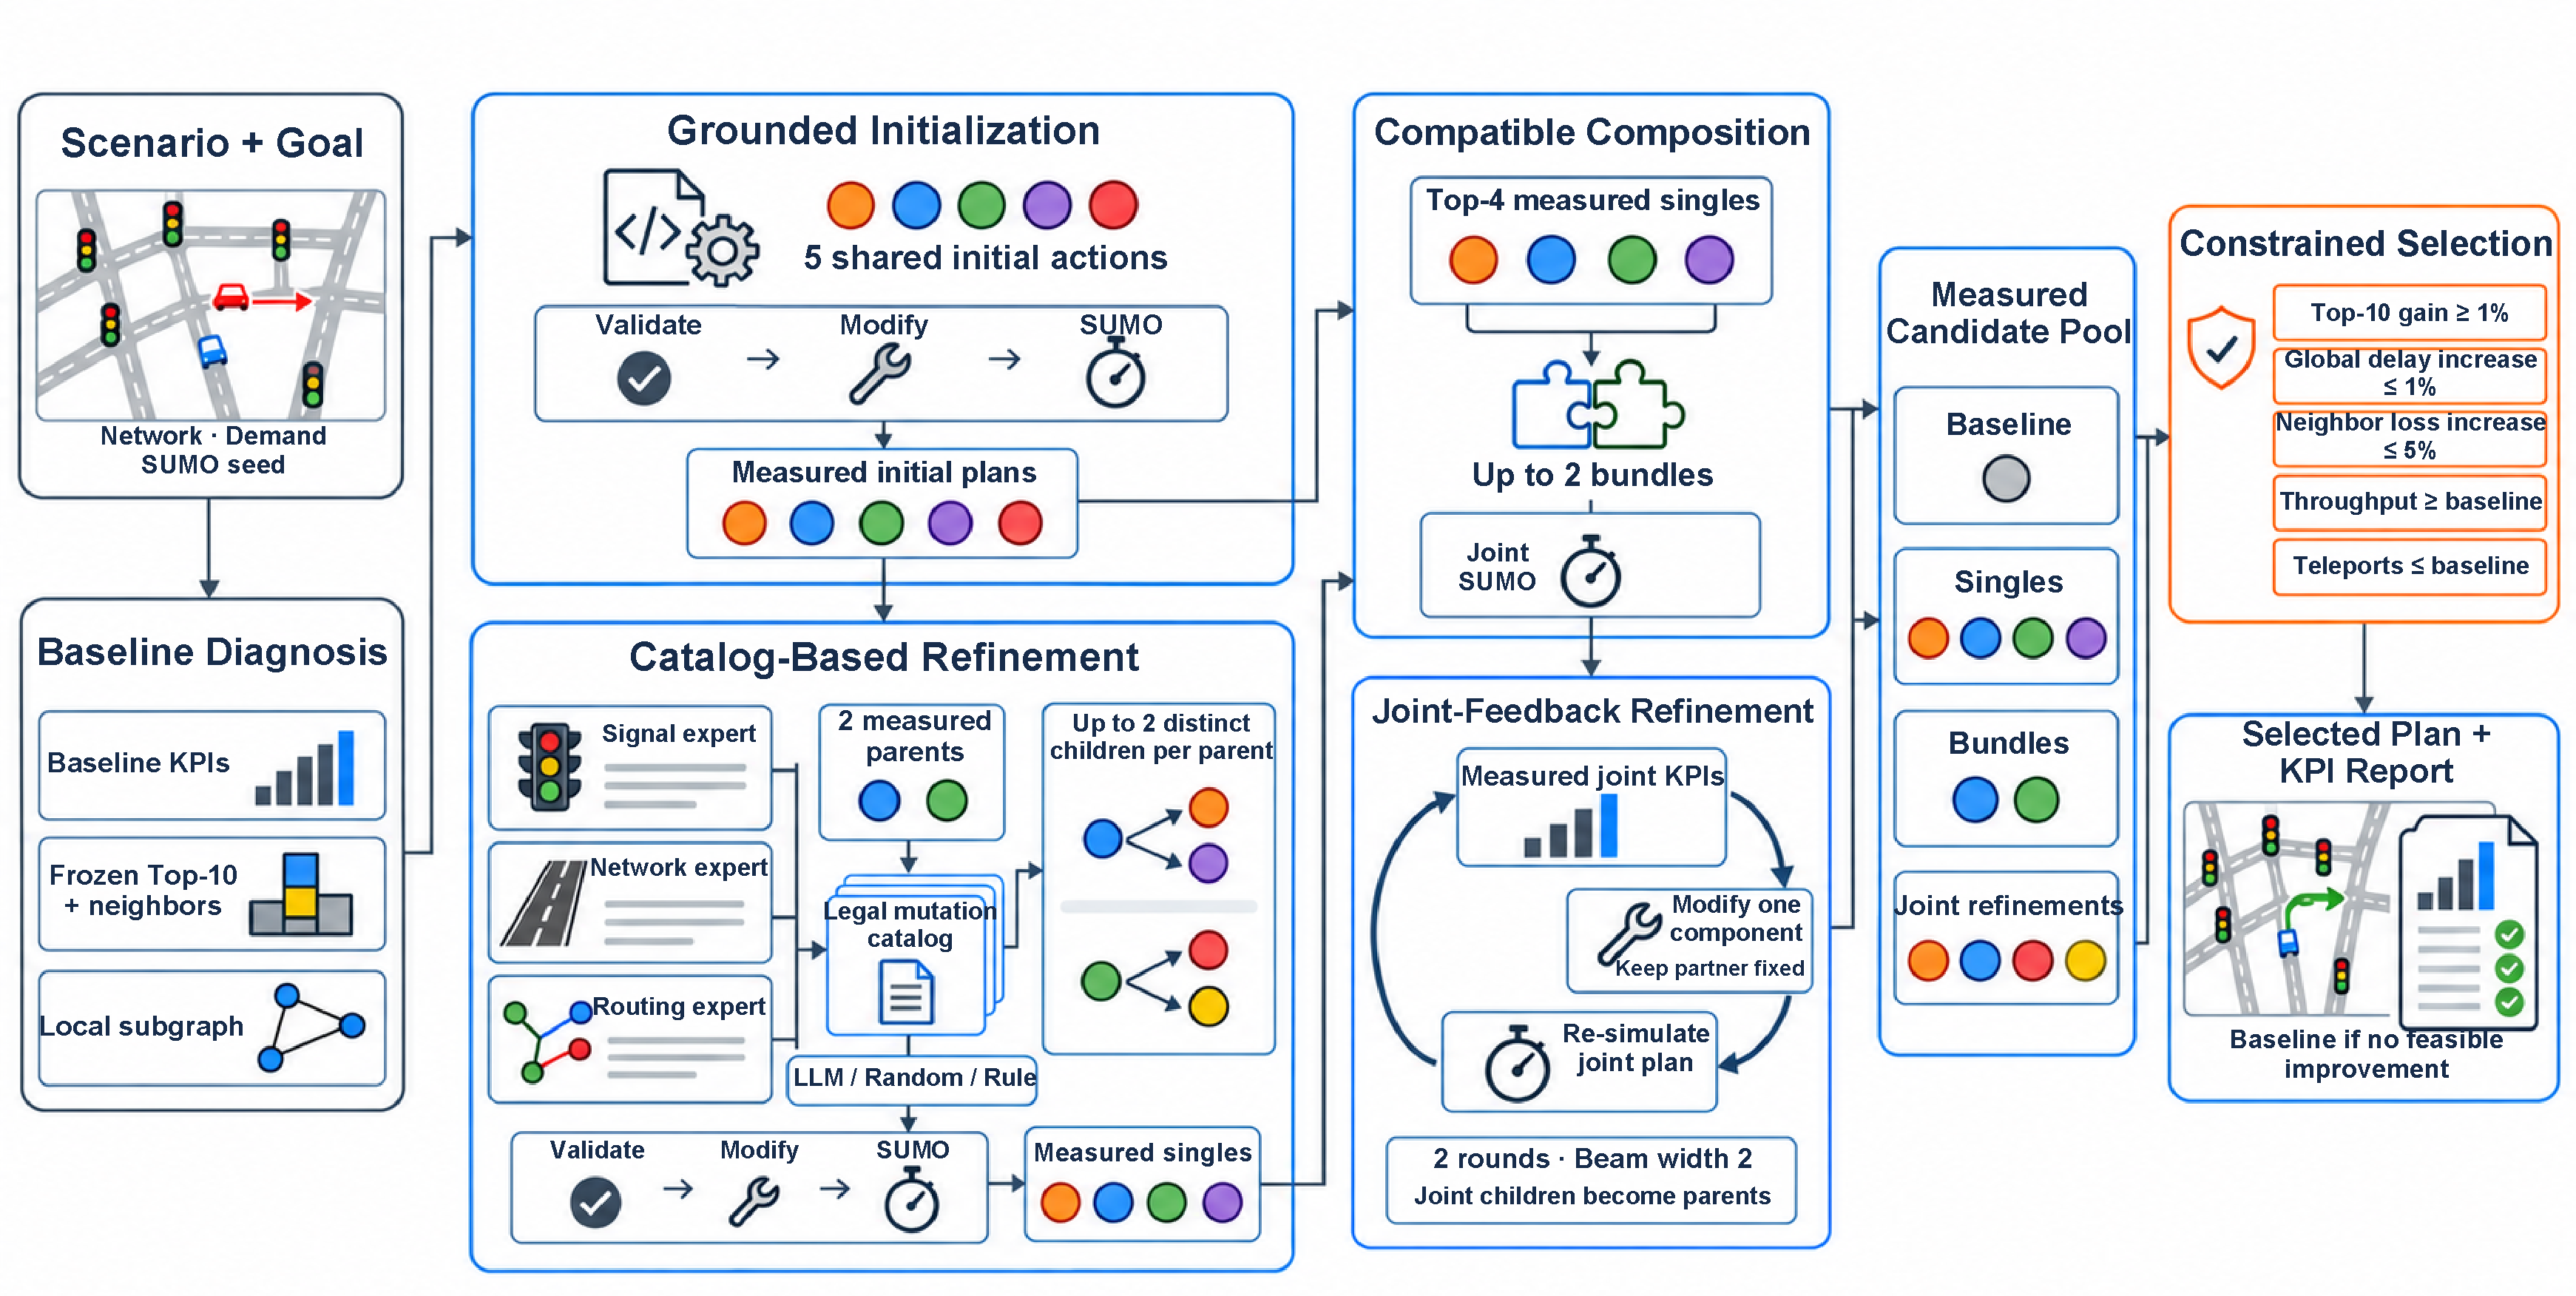
\includegraphics[width=\linewidth]{figures_current/Framework_updated.pdf}
\caption{SimTIO adaptive search: five shared initial actions, up to two children per measured parent, compatible bundles, and continued joint-feedback refinement. All selectors follow the same search rules; SUMO measurements and the explicit acceptance rule determine the retained plan. The schematic was created using OpenAI's image-generation tool through Codex, based on the authors' original framework illustration; labels were separately typeset in LuaLaTeX. The image tool did not expose a model/version identifier. Detailed rules are specified in Sections~\ref{sec:initialization}--\ref{sec:search}.}\label{fig:framework}
\end{figure}

\subsection{Frozen evidence and acceptance rule}
\label{sec:acceptance}
For baseline scenario $x_0$, SUMO produces trip-level time loss, completion counts, emissions, and edge measurements~\cite{lopez2018sumo}. The diagnosis ranks congested edges using the implemented congestion score and excludes fragments shorter than 10~m from objective candidates. The ten selected baseline edges form $T$; their one-hop neighbors outside $T$ form $N$. Both sets remain fixed throughout the search. They are not recomputed after an intervention.

Specifically, with $\phi(x;h)=\min(1,\max(0,x/h))$, the ranking score is $0.35[1-\phi(r_e;1)]+0.25\phi(\rho_e;35)+0.20\phi(o_e;30)+0.10\phi(L_e;300)+0.10\phi(W_e;300)$, where $r_e$ is the observed-to-limit speed ratio, $\rho_e$ density, $o_e$ occupancy, and $L_e,W_e$ accumulated time loss and waiting time. The diagnostic subgraph uses up to five seed edges, one hop, and an 80-edge limit. Candidate diagnostics can be recomputed for reporting, but the baseline target set remains unchanged.

For plan $p$, let $L_T(p)$ and $L_N(p)$ be sums of edgeData \texttt{timeLoss} over the respective edges and recorded intervals. This SUMO attribute is total vehicle time lost on the edge, not mean edge travel time~\cite{sumoEdgeData}. Let $D(p)$ be mean trip time loss, $q(p)$ the completed-demand fraction, and $h(p)$ the teleport count. Define
\begin{align}
R_T(p)&=1-L_T(p)/L_T(x_0),\\
\Delta_D(p)&=D(p)/D(x_0)-1,\qquad
\Delta_N(p)=L_N(p)/L_N(x_0)-1.
\end{align}
The default acceptance conditions are
\begin{equation}
R_T(p)\geq 0.01,\quad \Delta_D(p)\leq0.01,\quad
\Delta_N(p)\leq0.05,\quad q(p)\geq q(x_0),\quad h(p)\leq h(x_0).
\label{eq:acceptance}
\end{equation}
Demand and OD preservation are checked during intervention execution. These conditions are engineering screening tolerances, not statistically derived significance thresholds or guarantees of transport safety. If the neighbor denominator is unavailable, the implementation omits that relative check and records availability; the analyzed candidate logs contain the necessary scope KPIs. Among accepted plans, selection minimizes $L_T$. A normalized weighted KPI score breaks ties, followed by preference for the baseline. The baseline is always eligible and yields zero improvement if no intervention passes.


\subsection{Grounded initialization and executable validation}\label{sec:initialization}
The full adaptive protocol draws five distinct initial proposals with a seeded grounded sampler. Specialist roles cycle through signal, network, routing, signal, and network; within each role an available action family and validated parameter configuration are sampled. The first three draws are shared with the smaller controlled protocol. All five actions are frozen before the two additional measurements; they are not chosen using subsequent mutation or bundle outcomes. Signal targets come from the diagnosed subgraph; other targets use diagnosed objective edges. Initial corridor factors are $\{0.7,0.8,0.9\}$ and rerouting fractions are $\{0.25,0.5,0.75,1\}$. Rerouting uses one avoided edge. A requested five-edge corridor can be shorter where connected same-road segments end.

Validation checks action registration, required artifacts and parameters, numeric ranges, target identifiers, and action-specific capability. Signal validation checks the actual traffic-light inventory and adjustable green phases; network actions check valid targets, corridor speeds, or bypass availability. Routing catalog validation does not guarantee that an alternative route exists. Route rebuilding and preservation of vehicles and OD endpoints are checked during execution. An argument-valid proposal can therefore fail before simulation or become infeasible after execution; such outcomes are retained without replacement.

Each intervention uses isolated files. Signal optimization preserves phase states and intergreen durations, allocating available green time in proportion to route-derived phase-demand estimates subject to a minimum share. Existing green durations are used when demand estimates are unavailable. The default cycle is 90~s and minimum share 0.08; this is not Webster cycle optimization. Rerouting retains demand and original OD pairs, while corridor control modifies static simulation speed limits. These tools require additional behavioral and engineering validation before practical use.

\subsection{Finite mutation catalogs}\label{sec:catalog}
Figure~\ref{fig:intervention-mechanisms} illustrates three supported intervention mechanisms. These are scenario-editing operations; the displayed schematic parameters are not measurements or a universal parameter prescription.

\begin{figure}[htbp]\centering
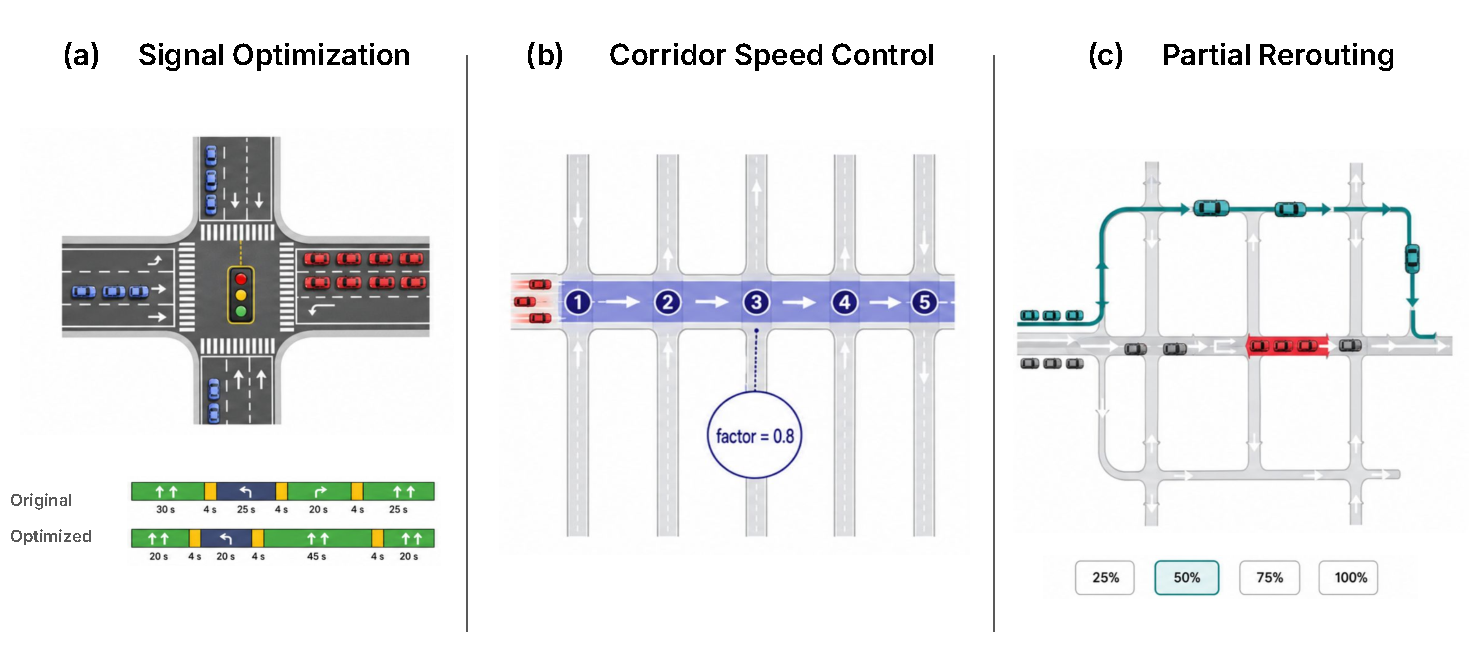
\includegraphics[width=\linewidth]{figures_current/intervention_mechanisms_original.pdf}
\caption{Illustrative intervention mechanisms: (a) signal green-time reallocation, (b) corridor speed-limit adjustment, and (c) partial rerouting. Durations, speed factor, and rerouting percentages are schematic annotations, not settings or observed effects from the reported cases. Actual parameters are specified by the executable tools and legal catalogs; the figure does not depict every supported network-editing action.}\label{fig:intervention-mechanisms}
\end{figure}

The catalog builder starts from a measured parent, retains its action family, and changes exactly one non-path argument. Artifact paths are bound by the orchestrator. Candidate construction is deterministic given the parent, diagnosis, feedback, and evaluated-history set. Table~\ref{tab:catalog} specifies the implemented enumeration; generic mutable-field declarations do not imply that every declared field is enumerated.

\begin{table}[htbp]
\centering\small
\caption{Actual catalog enumeration. Every proposed change passes the same executable validator before inclusion.}\label{tab:catalog}
\begin{tabular}{p{.19\linewidth}p{.72\linewidth}}
\toprule Family & Enumeration and order \\
\midrule
Signal & Alternative cycles in $\{75,90,105\}$~s, ordered by distance from the current value, then value; minimum shares in $\{.05,.08,.12\}$ similarly; then legal TLS targets in diagnosed order. Offset is not enumerated. \\
Corridor speed & Alternative factors in $\{.7,.8,.9\}$, ascending for a parent without safeguard violations and descending when global delay, neighbor spillover, throughput, or teleports fail; then alternative objective-edge anchors. Edge count is fixed. \\
Rerouting & Alternative fractions in $\{.25,.5,.75,1\}$; when safeguards fail, smaller fractions precede larger ones, with nearest changes first; otherwise larger fractions precede smaller ones. Then single alternative objective-edge targets. \\
Edge removal & Alternative validator-confirmed removal targets in the legal network pool. \\
One-way conversion & Alternative legal retained-edge targets only when no explicit opposite-edge identifier would become stale. \\
\bottomrule
\end{tabular}
\end{table}

The builder rejects unchanged or multi-field proposals, validator failures, and signatures already present in the measured history or current catalog. Signatures contain the action and semantic arguments, excluding file paths and explanatory text. The catalog stops at 24 accepted entries. IDs are assigned sequentially \emph{after} filtering; consequently, the same ID in different catalogs need not denote the same action. The implementation records complete ordered semantic catalogs, SHA-256 fingerprints, proposed changes, validation results, and rejection reasons. Full catalogs and filter audits are saved directly for the reported experiments; matching IDs alone is not treated as evidence of matching semantic actions.

Validator ranges are distinct from enumeration choices: a cycle must be positive; minimum green share must lie in $(0,0.5)$; corridor factors must lie in $[0.70,0.95]$ and requested edge count must be an integer in $[2,10]$. Routing accepts one to three distinct avoided-edge IDs, the four stated fractions, and complete route retention; the experiment narrows this to one avoided edge. At execution, fixed intergreen time must leave positive green time and resulting phase durations must remain positive. These checks do not certify pedestrian clearance or corridor coordination.


\subsection{Two children from each measured parent}\label{sec:children}
Parent selection retains up to two successfully simulated initial plans, preferring final-selection feasibility, the number of satisfied checks, and Top-10 score; role diversity is preferred before filling the remaining positions. Each specialist receives the parent, diagnosis, measured feedback, initial-only history, and ordered legal catalog. It selects a mutation ID; the orchestrator resolves that ID to executable arguments. Natural-language benefit claims do not enter the acceptance rule.

In the full protocol, each parent produces two distinct children. Both directly modify the original parent and use the same initial-only history and parent feedback. The second request excludes the first selected semantic action while preserving the remaining IDs and ordering. It does not use the first child's KPI. Cross-parent duplicates are not simulated again and do not receive replacement draws. This widens exploration without turning siblings into a sequential refinement chain. The first request per parent is identical across selectors; the remaining sibling catalog can differ because of the first choice.

\subsection{Composition and continued joint feedback}\label{sec:search}
Up to two compatible pairs are generated from the four highest-ranked successfully simulated single interventions. Pair priority uses the sum of negative single-plan Top-10 scores followed by compatibility and action-order rules. Ranking does not first exclude singles that violate final safeguards. Each pair is rebuilt from the baseline and executed in order, with validation against the intermediate artifacts and one simulation of the completed composition.

Measured bundles become candidates for two additional feedback rounds with beam width two. A role-specific specialist changes one field of one component conditional on the measured whole-plan feedback, while its partner remains fixed. Component ownership rotates along each root lineage; exhausted component catalogs can be skipped. Joint deduplication uses the full ordered pair, so a component already tested alone can still be tested with a different partner. Joint children can become parents in the next round. Every child is rebuilt from the baseline; accepting a single component does not establish that the joint plan is feasible. The primary experiments use aggregate joint feedback, not an inferred additive decomposition of component effects.

The full cap is 15 candidate evaluations: five initials, up to four single mutations, two bundles, and four joint refinements. Baseline measurement is separate. Cache reuse consumes the same logical budget as simulation. A simulation that runs and then fails a feasibility check consumes budget; rejection before SUMO does not. Unused slots are not filled with extra samples. The top-four compatibility rule can prevent bundle formation even when lower-ranked singles would form a legal pair; we preserve and audit this limitation across all selectors.

\section{Experimental design and reproducibility}\label{sec:design}
OpenAI Codex assisted with implementation changes, experiment execution, analysis scripts, and data-derived visualizations. Reported tables and plots are generated from saved simulation and selection records using the documented analysis procedures. The authors reviewed and approved the manuscript and take responsibility for the reported work. This development assistance is distinct from the LLM selector evaluated below.

\subsection{Networks, synthetic demand, and execution audit}\label{sec:demand}
Five OpenStreetMap-derived extracts~\cite{openstreetmap} are evaluated with 2,400 passenger trips departing over one hour, generated using \texttt{randomTrips.py} 1.24.0. Demand and SUMO seeds are 42, 43, and 44. The fixed demand file, network, and simulation seed are shared across methods within each case. Table~\ref{tab:networks} describes the instances rather than calibrated city traffic.

\begin{table}[htbp]\centering\small
\caption{Network inventory and baseline mean trip time loss (mean $\pm$ sample SD over three seeds). Junction totals include internal records.}\label{tab:networks}
\begin{tabular}{lrrrr}
\toprule
Network & External edges & Junctions & TLS & Delay (s) \\
\midrule
Albany & 6193 & 4309 & 107 & 112.80 $\pm$ 0.26 \\
Ann Arbor & 10151 & 7522 & 81 & 138.58 $\pm$ 3.13 \\
Los Angeles & 6969 & 4954 & 172 & 175.76 $\pm$ 1.26 \\
Manhattan & 5993 & 4065 & 256 & 245.31 $\pm$ 13.03 \\
Troy & 6107 & 4355 & 57 & 99.79 $\pm$ 0.84 \\
\bottomrule
\end{tabular}

\end{table}

Execution uses SUMO 1.27.1. An implementation audit found that an older rerouting configuration writer could omit the simulation seed and additional files. Configuration inheritance was repaired; the reported measurements are audited using the executed configuration embedded in tripinfo, not directory labels. Frozen inputs include file hashes. Fresh feedback and parent catalogs for the corrected three-initial experiment were reconstructed from seed-verified initial measurements. The earlier short-output model diagnostic is also superseded: the current completion cap is 4,096 tokens, rather than 500. Results from those earlier implementations are not pooled with the reported cohorts.

\subsection{Controlled selector comparison and adaptive search}\label{sec:matched}
We use two distinct endpoints. First, a \emph{frozen-input comparison} holds three initial proposals and measurements, two parents, complete ordered catalogs, initial-only history, SUMO seed, and bundle rules constant. Each parent receives one mutation, selected by the LLM, uniformly from the catalog, or by taking the first entry in its feedback-dependent deterministic ordering. Earlier selections cannot change the second parent's information or catalog. Up to two bundles follow, giving a cap of seven evaluations. This endpoint is retrospectively extracted from the saved pre-joint stage of the corrected three-initial experiment. Later joint outcomes are excluded; extraction does not create a new independent cohort or require new model calls. Both parent requests are verified identical across arms by content hashes.

Second, the \emph{adaptive search} applies the full five-initial, two-child, joint-feedback procedure with cap 15. Fifteen city--seed cases are each evaluated once per selector. Initial proposals, parents, base catalogs, simulator settings, and search rules are shared. Sibling exclusions and subsequent joint parents may diverge as a consequence of selection. This is a comparison of selector policies inside a common adaptive procedure, not a claim that every future catalog remains identical. Comparing its endpoint with the seven-budget endpoint does not isolate search width, depth, or the value of joint feedback.

LLM calls use \texttt{gpt-5.6-luna}, JSON response mode, default sampling, and a 4,096-completion-token cap. The configured and returned model identifiers, finish reasons, token usage, exact requests, and responses are logged. No model sampling seed is specified. Infrastructure failures are separately recorded and retried after connectivity is restored; failed model decisions would remain failed without a rule-based substitute. Random selection uses $20260927+s+1000r+j$, where $s$ is SUMO seed, $r$ repeat index, and $j$ request index. The rule is a substantive comparator because catalog ordering already encodes conservative responses to failed safeguards. Semantic simulation caches are consulted only after selecting an action and never supply unseen feedback to the search.

\subsection{Fixed-demand sampling stability}\label{sec:stability}
For all five networks at seed 42, LLM and random searches are repeated five times; the deterministic rule is evaluated once. Existing repeat zero is retained, adding 40 complete searches. Demand, five initial actions, parent measurements, and base catalogs remain fixed. We report within-city sample SD, range, feasibility, and the mutation-frequency distribution of each parent's first child. Those first-child requests provide a strictly identical-input sampling comparison. Sibling and later joint requests can diverge, and are not pooled as if they shared a catalog. Repeats are nested within cases, not counted as additional cities. Reuse of an earlier repeat and an unversioned returned model identifier means undisclosed provider changes cannot be excluded.

\subsection{Demand-intensity sensitivity}\label{sec:demand-sensitivity}
Albany and Manhattan are preselected as contrasting network scales. Each uses seeds 42--44 at 1,200, 2,400, and 3,600 trips over the same $[0,3600)$-s departure window. The six 2,400-trip cases reuse the adaptive experiment. For each archived demand, seeded sampling selects one trip from every adjacent departure pair. Those 1,200 original trips form low demand. High demand retains all 2,400 originals and adds those same 1,200 OD pairs with unique IDs and departures shifted by 0.75~s; all other vehicle attributes are preserved. This paired construction limits OD-regeneration differences but does not exactly preserve empirical OD shares at every level.

Each new scenario receives a new baseline, frozen Top-10 set, diagnosis, and five initial actions. All actions are frozen before measurement and shared across selectors. Twelve new baselines and 36 new complete searches are added, with one search sample per method/scenario. SUMO continues until trips are recorded as completed, which can include teleport recovery. Percentages across demand levels can concern different target edges and baseline losses. These are synthetic intensity tests, not calibration to observed flows or OD data.

\subsection{Thresholds, spatial diagnostics, and statistics}\label{sec:statistics}
Saved candidate KPIs are reselected over 100 settings: minimum Top-10 reductions $\{0,0.5,1,2,5\}$\%, maximum global-delay increases $\{0,0.5,1,2,5\}$\%, and maximum neighbor increases $\{0,2.5,5,10\}$\%. Throughput, teleports, and demand preservation remain constrained. Reselection changes the retained plan within an already measured pool; it does not model how changed thresholds would alter the search itself.

Over the union of observed edges in each baseline and retained plan, we calculate signed accumulated time-loss changes, the fraction worsening, and the 95th percentile. Outside $T\cup N$ we record the largest edge increase, total positive increases, edges worsening by over 60 vehicle-seconds, and the largest net increase in fixed 500-m projected-coordinate cells. Edges absent under \texttt{excludeEmpty=true} contribute zero accumulated loss for that run. This does not imply free-flow travel. Topological remoteness is distinguished from geographic distance; worst-edge records also give Euclidean distance to the nearest target edge using the mean coordinates of each edge's shape vertices. The same representative coordinates assign edges to 500-m cells; they are not necessarily geometric midpoints.

All final outcomes, including no-op with zero improvement, enter summaries. City--seed cases are paired across methods. We report two-sided exact sign-flip tests and Wilcoxon tests using nonzero differences, a normal approximation, and no continuity correction. The two LLM comparisons within each protocol, or within each demand level, receive Holm adjustment. City-level sign-flips and 20,000 city-cluster bootstrap draws (seed 20260927) address within-city dependence, although only five cities---and two for demand sensitivity---limit inference. Stability comparisons first average repeats within each city. SD describes dispersion, not a confidence interval. Candidate edges and repeated model calls are not treated as independent transport scenarios.

\section{Results}\label{sec:results}
\subsection{Selector comparison and full adaptive search}\label{sec:main-results}
Table~\ref{tab:main} separates the controlled prefix from the adaptive endpoint. Under frozen parent/catalog inputs, LLM mean Top-10 improvement is \StrictLLMTop\%, versus \StrictRuleTop\% for the rule and \StrictRandomTop\% for random selection. All arms use 103 logical evaluations across 15 cases. The 30 LLM mutation requests succeed; the differences therefore cannot be attributed to the former short-output failure mode. Paired mean differences are $-0.86$ and $-1.05$ percentage points (pp), with no evidence of LLM superiority (Table~\ref{tab:paired}).

\begin{table}[htbp]\centering\small
\caption{Separate protocol endpoints over the same 15 city--seed cases. Top-10 entries are mean $\pm$ sample SD; global is mean percentage reduction in trip time loss. Evals counts actual logical candidate evaluations, including cache reuse. No-ops remain in the denominator.}\label{tab:main}
\begin{tabular}{llrrrr}
\toprule
Protocol (cap) & Selector & Top-10 (\%) & Global (\%) & Success & Evals \\
\midrule
Frozen prefix (7) & LLM & 8.50 $\pm$ 10.37 & 2.48 & 12/15 & 103 \\
Frozen prefix (7) & Rule & 9.36 $\pm$ 10.18 & 2.82 & 14/15 & 103 \\
Frozen prefix (7) & Random & 9.55 $\pm$ 11.18 & 2.60 & 13/15 & 103 \\
Adaptive search (15) & LLM & 11.53 $\pm$ 10.57 & 3.17 & 13/15 & 203 \\
Adaptive search (15) & Rule & 12.10 $\pm$ 11.07 & 3.22 & 13/15 & 199 \\
Adaptive search (15) & Random & 14.81 $\pm$ 10.55 & 3.37 & 13/15 & 210 \\
\bottomrule
\end{tabular}

\end{table}

The full adaptive search yields \WideLLMTop\%, \WideRuleTop\%, and \WideRandomTop\% mean reduction, respectively. Each method finds a feasible plan in 13/15 cases. Relative to the rule and random selector, the LLM's paired differences are $-0.57$ and $-3.28$ pp. The random comparison has an exact case-level $p=0.078$, city-level $p=0.125$, and Holm-adjusted Wilcoxon $p=0.169$. Failure to reject does not establish equivalence; the point estimates do not favor the LLM. Its descriptive city-bootstrap interval against random is $[-6.58,-0.51]$ pp, while the discrete city-level test does not reject. Five clusters do not support precise confirmatory interval claims.

\begin{table}[htbp]\centering\small
\caption{Paired Top-10 differences. Positive differences favor LLM. Exact sign-flip tests are reported at case and city levels; $p_W$ is Holm-adjusted Wilcoxon within each protocol's two comparisons.}\label{tab:paired}
\begin{tabular}{llrrrr}
\toprule
Protocol & LLM minus & $\Delta$ (pp) & $p_{\mathrm{case}}$ & $p_{\mathrm{city}}$ & Holm $p_W$ \\
\midrule
Frozen prefix & Rule & -0.86 & 0.438 & 0.375 & 0.569 \\
Frozen prefix & Random & -1.05 & 0.386 & 0.500 & 0.569 \\
Adaptive search & Rule & -0.57 & 0.727 & 0.750 & 0.530 \\
Adaptive search & Random & -3.28 & 0.078 & 0.125 & 0.169 \\
\bottomrule
\end{tabular}

\end{table}

The adaptive cohort uses 612 logical evaluations: 225 newly executed candidate simulations, including 22 shared additional-initial simulations, and 387 cache uses. All 108 LLM requests finish with valid selections. Ten earlier DNS transport faults are separately logged. Nine of 45 searches form no initial bundle because their top-four singles lack a compatible pair. All nine have a compatible pair when the entire measured single pool is considered, but those alternatives were not simulated. The actual counts are therefore below the nominal $45\times15$ cap.

Figure~\ref{fig:proposal-source-comparison} disaggregates adaptive outcomes by network and contrasts case success with the share of evaluated candidates satisfying the acceptance rule. The latter counts cache reuse and is not a measure of newly executed SUMO efficiency. Figure~\ref{fig:proposal-source-actions} shows the final plan families and the origin of selected LLM plans: three initial singles, five refined singles, two initial bundles, three joint-refined bundles, and two no-ops. Plan origin describes the selected trajectory; it does not establish the causal value of an additional search stage.

\begin{figure}[htbp]\centering
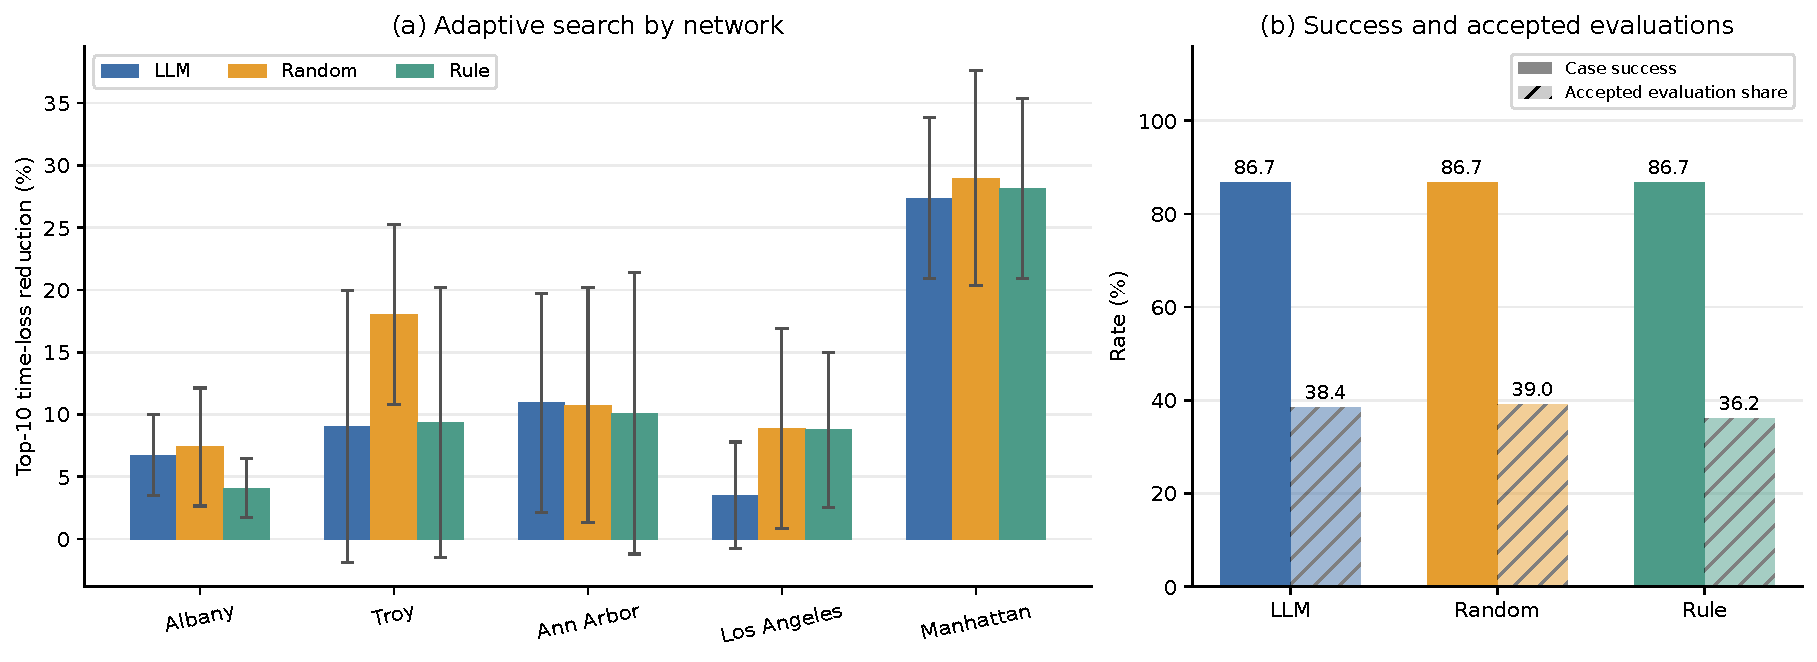
\includegraphics[width=\linewidth]{figures_current/proposal_source_comparison_current.pdf}
\caption{Adaptive selector comparison. (a) Network means and sample SD over seeds 42--44, including no-op outcomes. (b) Feasible-plan success over 15 cases and accepted-evaluation shares of 78/203, 82/210, and 72/199 for LLM, random, and rule selection, respectively. Each selector succeeds in 13/15 cases. Shared initial candidates are counted within each search; candidate-level shares are descriptive, not independent statistical replicates.}\label{fig:proposal-source-comparison}
\end{figure}

\begin{figure}[htbp]\centering
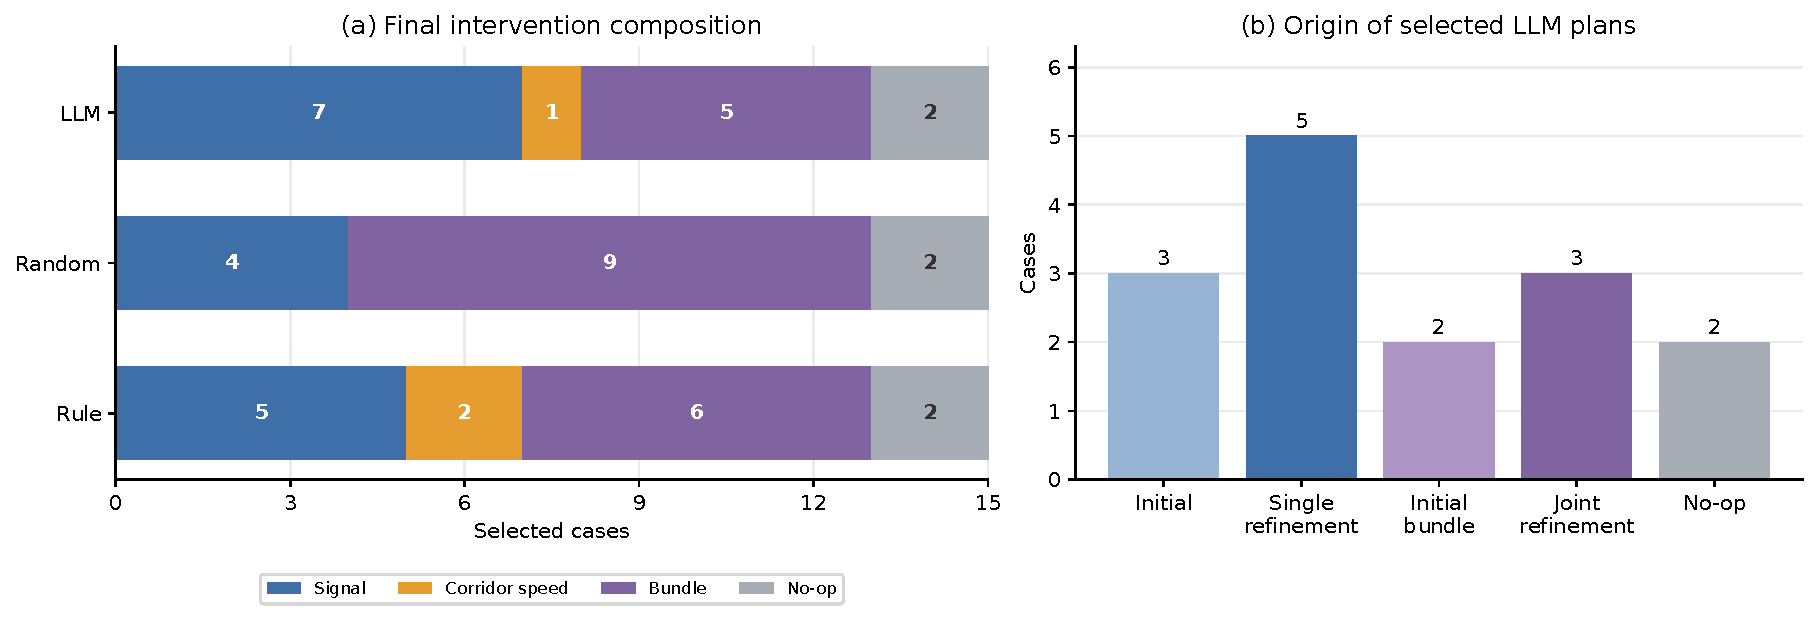
\includegraphics[width=\linewidth]{figures_current/proposal_source_action_distribution_current.pdf}
\caption{Selected plans in the current adaptive cohort, 15 cases per selector. (a) Final intervention family; the bundle category includes both initial compositions and jointly refined descendants. (b) Origin of the final LLM plan, separating initial bundles from continued joint refinement. No-op cases remain explicit.}\label{fig:proposal-source-actions}
\end{figure}

Before joint refinement, adaptive LLM, rule, and random mean improvements are 10.88\%, 11.81\%, and 11.96\%; final means increase by 0.65, 0.29, and 2.84 pp (Figure~\ref{fig:adaptive}). These are within-search stage changes, with best-plan retention. They are not an equal-budget comparison against spending those additional slots on independent exploration.

\begin{figure}[htbp]\centering
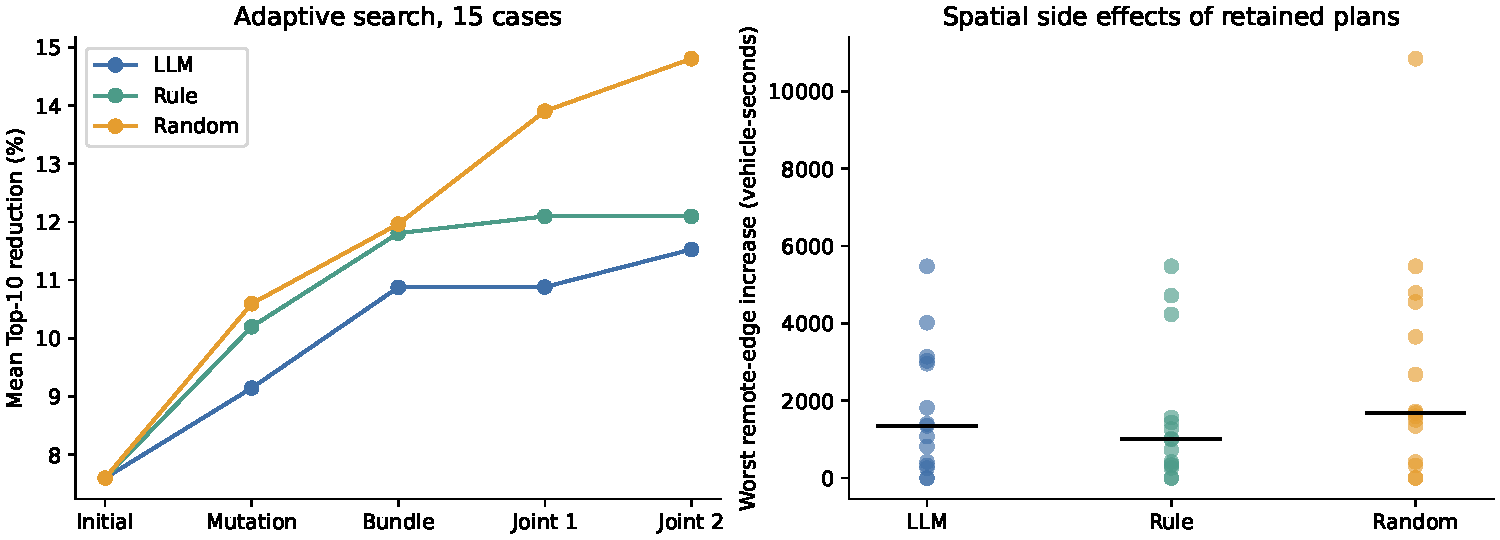
\includegraphics[width=\linewidth]{figures_current/adaptive_search.pdf}
\caption{Adaptive search. Left: retained improvement by measured stage, averaged over the 15 cases. Right: worst remote-edge increase in each retained result; black bars are medians and no-op outcomes remain at zero.}\label{fig:adaptive}
\end{figure}

\subsection{Sampling variation under fixed demand}\label{sec:stability-results}
The five-city stability subset has LLM, rule, and random mean improvements of 14.60\%, 16.61\%, and 15.43\%. These seed-42 subset means do not replace the 15-case primary means. LLM performance ranges from 8.07\% to 22.31\% in Ann Arbor and 8.27\% to 19.74\% in Los Angeles (Table~\ref{tab:stability}). Mean within-city SD is 3.09 pp for LLM and 2.55 pp for random search. LLM choices vary for seven of ten identical initial-parent catalogs; random choices vary for all ten.

\begin{table}[htbp]\centering\small
\caption{Fixed-demand stability. All improvements are percentages; LLM and random have five repeats per city, the rule one evaluation. SD is within-city sampling dispersion.}\label{tab:stability}
\begin{tabular}{lrrrr}
\toprule
Network & LLM mean $\pm$ SD & LLM range & Random mean $\pm$ SD & Rule \\
\midrule
Albany & 3.24 $\pm$ 0.60 & 2.98--4.31 & 3.24 $\pm$ 0.60 & 2.98 \\
Ann Arbor & 16.15 $\pm$ 6.83 & 8.07--22.31 & 15.95 $\pm$ 3.83 & 22.31 \\
Los Angeles & 12.86 $\pm$ 6.28 & 8.27--19.74 & 15.57 $\pm$ 3.26 & 14.42 \\
Manhattan & 34.71 $\pm$ 0.79 & 33.89--35.47 & 37.44 $\pm$ 2.24 & 36.50 \\
Troy & 6.04 $\pm$ 0.97 & 4.47--6.85 & 4.94 $\pm$ 2.81 & 6.85 \\
\bottomrule
\end{tabular}

\end{table}

LLM and random searches succeed in 25/25 runs, and the rule in 5/5 cases. Every shared initial set already contains a feasible plan, so best-plan retention creates a success-rate ceiling. These counts do not demonstrate robust generation or a better selector. No model-output failure is observed in the added 160 LLM requests, but five repeats provide limited evidence about rare failure probabilities. Paired comparisons of city means give LLM-minus-rule and LLM-minus-random differences of $-2.01$ and $-0.83$ pp, with exact city sign-flip $p=0.125$ and $0.500$. The added searches use 568 logical evaluations, of which 119 are new simulations and 449 cache reuse. The supplementary evidence contains all outcomes and choice frequencies.

\subsection{Dependence on synthetic demand intensity}\label{sec:demand-results}
Table~\ref{tab:demand} shows that relative mean performance depends on demand. At 1,200 trips the LLM has the largest mean reduction and succeeds in five of six cases, compared with four for each control. Its paired differences are $+8.65$ pp versus the rule and $+4.13$ pp versus random, but exact case sign-flip $p$ values are 0.125 and 0.313. At 2,400 and 3,600 trips random has the highest mean. These small two-city comparisons do not establish a universal ordering.

\begin{table}[htbp]\centering\small
\caption{Synthetic intensity sensitivity: six city--seed cases per level, one search per method/scenario. SD is across cases; 2,400-trip rows reuse the corresponding primary cases.}\label{tab:demand}
\begin{tabular}{rlrrr}
\toprule
Trips & Selector & Top-10 mean $\pm$ SD (\%) & Success & Global (\%) \\
\midrule
1200 & LLM & 16.93 $\pm$ 13.76 & 5/6 & 2.57 \\
1200 & Rule & 8.27 $\pm$ 9.62 & 4/6 & 0.67 \\
1200 & Random & 12.80 $\pm$ 11.55 & 4/6 & 1.73 \\
2400 & LLM & 17.05 $\pm$ 12.19 & 6/6 & 6.40 \\
2400 & Rule & 16.12 $\pm$ 14.03 & 6/6 & 5.80 \\
2400 & Random & 18.19 $\pm$ 13.36 & 6/6 & 6.34 \\
3600 & LLM & 8.75 $\pm$ 12.00 & 4/6 & 0.56 \\
3600 & Rule & 6.98 $\pm$ 8.93 & 4/6 & 0.81 \\
3600 & Random & 8.81 $\pm$ 11.97 & 4/6 & 0.44 \\
\bottomrule
\end{tabular}

\end{table}

Manhattan's 3,600-trip baselines have 84, 93, and 100 teleports at seeds 42, 43, and 44, respectively. The retained LLM outcomes have 60, 93, and 84; the middle case is no-op. Such completion includes simulator teleport recovery rather than uninterrupted physical trips. The unchanged constraint limits teleports relative to each baseline, not to zero. These high-demand outcomes must therefore be interpreted as congested simulation stress tests, and their apparent delay reductions are qualified accordingly. Baseline congestion changes much more in Manhattan than Albany (Figure~\ref{fig:demand}), illustrating why equal trip counts do not imply comparable operating conditions.

\begin{figure}[htbp]\centering
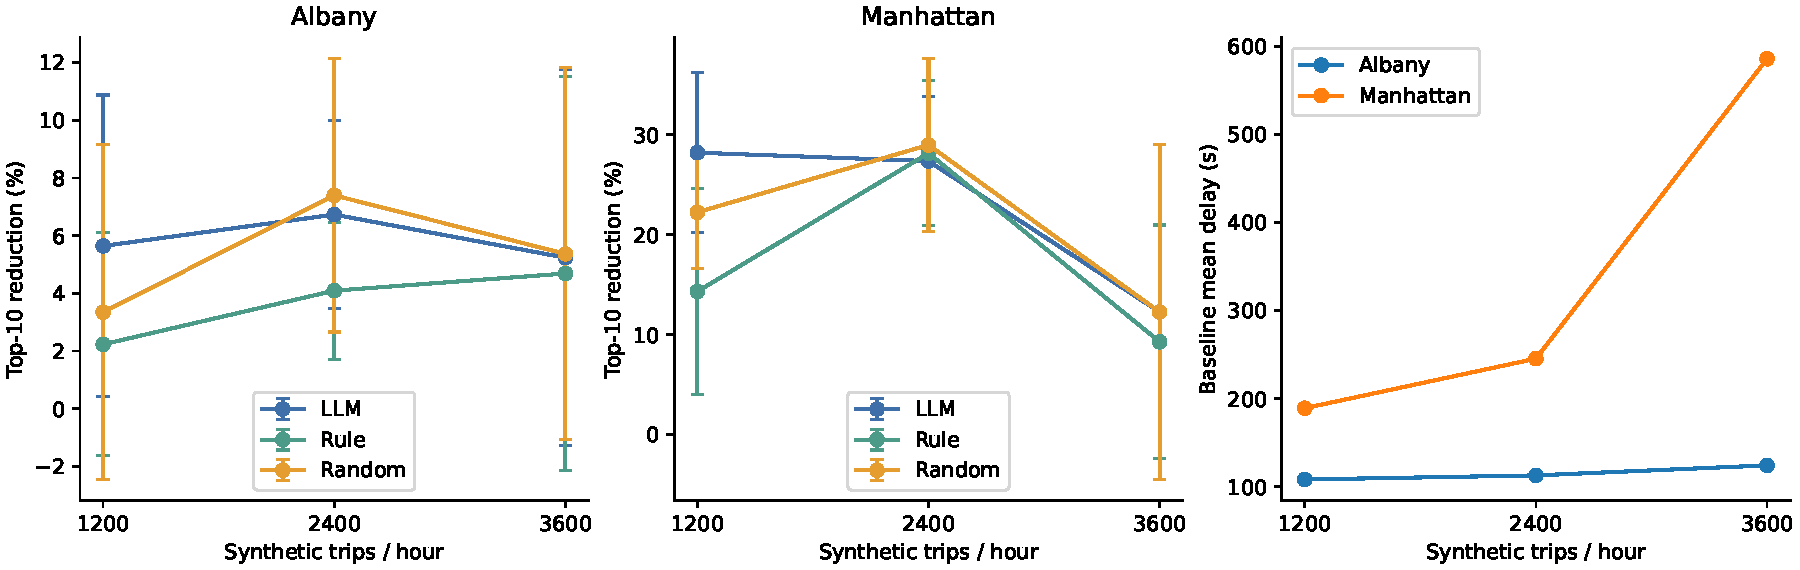
\includegraphics[width=\linewidth]{figures_current/demand.pdf}
\caption{Demand sensitivity by city and baseline congestion. Error bars are SD over three seeds, not confidence intervals. Targets are re-frozen for each demand scenario.}\label{fig:demand}
\end{figure}

The new demand searches use 489 logical candidate evaluations: 305 new simulations, counting shared initialization once, and 184 cache uses, plus twelve baseline simulations. All 88 new LLM requests complete successfully; eight transport faults are recorded separately. Candidate execution failures, including no available alternative route or lost demand, remain recorded and are not confused with model-output failures. One model sample at each new demand level cannot completely separate demand effects from sampling variability.

\subsection{Acceptance sensitivity and spatial side effects}\label{sec:sensitivity-results}
Within the adaptive cohort's saved pools, random selection has the highest mean Top-10 reduction in all 100 threshold settings. Success-rate ordering is less stable: allowing 10\% neighboring loss raises LLM and rule success to 14/15 while random remains at 13/15 (Table~\ref{tab:sensitivity}). Thus the mean ranking is robust on this grid for this cohort, while feasibility counts depend on the tolerance. Thresholds should not be selected retrospectively to favor a method. Supplementary repeats and demand cohorts have their own separately reported grids.

\begin{table}[htbp]\centering\small
\caption{Selected threshold settings for the adaptive cohort. Thresholds are percentages; entries show successes/15 and mean Top-10 reduction in parentheses. Throughput, demand, and teleport checks remain unchanged.}\label{tab:sensitivity}
\begin{tabular}{lrrrrr}
\toprule
$R_T\geq$ & $\Delta_D\leq$ & $\Delta_N\leq$ & LLM & Rule & Random \\
\midrule
1 & 1 & 5 & 13/15 (11.53) & 13/15 (12.10) & 13/15 (14.81) \\
1 & 0 & 5 & 13/15 (11.53) & 13/15 (12.10) & 13/15 (14.74) \\
1 & 1 & 0 & 12/15 (10.13) & 13/15 (11.20) & 12/15 (12.98) \\
1 & 1 & 10 & 14/15 (12.03) & 14/15 (12.38) & 13/15 (15.27) \\
2 & 1 & 5 & 13/15 (11.53) & 13/15 (12.10) & 13/15 (14.81) \\
\bottomrule
\end{tabular}

\end{table}

\label{sec:spatial-results}
All three selectors have 13 retained outcomes with at least one edge outside $T\cup N$ worsening by more than 60 accumulated vehicle-seconds. For LLM, the median case-level worst remote-edge increase is 1,350.3 vehicle-seconds, and the maximum is 5,478.7; its maximum remote-cell net increase is 9,081.1 (Table~\ref{tab:spatial}). These harms coexist with satisfying the default aggregate constraints. The threshold refers to accumulated loss across travelers and the run, not an extra 60 seconds per traveler. Spatial counts, distributions, and worst-edge locations are supplied for every retained result; edges are not independent statistical replicates.

\begin{table}[htbp]\centering\small
\caption{Remote deterioration in adaptive outcomes. Cases have at least one remote edge worsening by over 60 vehicle-seconds. Maxima and median maxima include no-ops; cell values concern fixed 500-m regions.}\label{tab:spatial}
\begin{tabular}{lrrrr}
\toprule
Selector & Cases & Median max edge (s) & Max edge (s) & Max cell (s) \\
\midrule
LLM & 13/15 & 1350.3 & 5478.7 & 9081.1 \\
Rule & 13/15 & 1001.7 & 5478.7 & 16617.3 \\
Random & 13/15 & 1681.1 & 10848.2 & 9029.5 \\
\bottomrule
\end{tabular}

\end{table}

\section{Discussion and transport application boundaries}\label{sec:discussion}
\subsection{What the evidence supports}
The controlled prefix attributes differences to mutation selection within fixed parent/catalog inputs and common bundle rules. It does not attribute all final improvement to language reasoning: initialization already supplies useful plans, catalog construction encodes domain knowledge, and simulation-based rejection determines admissibility. The full adaptive comparison evaluates selector policies within a common procedure, allowing their later trajectories to differ. Neither result establishes LLM superiority, and neither evaluates the incremental value of three specialist roles over a centralized LLM with identical evidence and budget.

Continued joint feedback makes compositions revisable rather than terminal. Its measured stage gains show that some additional candidates improve the retained plan, particularly under random selection. They do not establish that joint refinement is a better use of simulation budget than additional independent proposals. Similarly, the wider protocol changes both initialization and available budget. Equal-budget width-versus-depth and joint-versus-independent-exploration controls remain untested; we make no causal claim about those design choices.

The catalog and composition policy define much of the attainable search space. One-field mutations can remain near local optima, and a top-four pool can exclude all compatible pairs despite compatible lower-ranked alternatives. Broadening the pool or perturbation range is a plausible future experiment, not a hidden correction applied to one reported arm. A limited auxiliary pilot that exposed measured component-interaction evidence did not improve its five-case mean (11.69\% versus 11.81\% with aggregate feedback); it used a common earlier search prefix and is not part of the primary comparison. More detailed prompts alone should not be assumed to improve optimization.

\subsection{Operational and planning decisions}\label{sec:horizons}
Signal retiming and rerouting belong to operational or periodic planning decisions, subject to controller compatibility, pedestrian clearance, coordination, compliance, and route acceptability. Corridor speed changes are operational only where suitable variable-speed infrastructure and authority exist; otherwise they involve regulatory or planning decisions. Edge removal and one-way conversion are network-design, closure, or construction scenarios requiring access, emergency-route, accessibility, and demand-adaptation assessment. A common simulator interface does not make these actions interchangeable real-time controls.

Time loss also depends on the reference desired speed and available routes. A static speed-limit reduction can change that reference, so reduced time loss is not by itself proof of shorter travel time, improved accessibility, or greater welfare. Our analysis uses the logged objective consistently, but practical evaluation should add absolute travel times, reliability, access, safety, and distributional outcomes. Runtime/API latency and controller deployment are not evaluated here.

\subsection{External validity and distributed safeguards}\label{sec:limitations}
No usable observed traffic counts or calibrated OD matrix were found in the repository. Intensity sensitivity extends the tested synthetic conditions but cannot substitute for calibration or observed validation. Following established calibration principles~\cite{hollander2008calibration,wunderlich2019toolbox}, a practical extension should fit demand and behavioral parameters to observed traffic and assess performance against separate observations before interpreting intervention effects. The paired demand construction changes empirical OD shares slightly, and the high-demand Manhattan runs involve teleport recovery. Three demand seeds and five fixed-demand repeats provide limited coverage of traffic and model uncertainty. The API model identifier is not an immutable model snapshot. Transfer to new networks, demand distributions, and behavior assumptions remains unresolved.

The baseline/no-op guard protects only the defined acceptance criteria. It does not eliminate concentrated remote deterioration, certify safety, or establish equitable benefits. Additional screening could constrain critical corridors, worst-region loss, or network-wide tails, but the appropriate thresholds require an application context. This study diagnoses these limitations without retroactively claiming that the search enforced such safeguards.

The experiments concern uncalibrated passenger traffic on network extracts. No public-transport priority, pedestrian interaction, freight demand, mode choice, or multimodal accessibility benefit is evaluated. SimTIO is therefore positioned as a simulation scenario-screening framework across specified decision horizons, not a unified real-time traffic controller or evidence of actual city-level improvement.

\section{Conclusions}\label{sec:conclusions}
SimTIO integrates grounded candidate generation, legal mutation catalogs, executable validation, intervention composition, and continued joint-feedback refinement under explicit simulation constraints. The controlled selector endpoint yields mean Top-10 reductions of \StrictLLMTop\%, \StrictRuleTop\%, and \StrictRandomTop\% for LLM, rule, and random selection. The full adaptive protocol yields \WideLLMTop\%, \WideRuleTop\%, and \WideRandomTop\%, with identical success counts of 13/15. Neither comparison establishes an LLM advantage.

Repeated searches expose conditional outcome variability, demand sensitivity changes relative performance, and remote-edge diagnostics show that aggregate acceptance does not ensure spatially uniform benefit. The supported contribution is an auditable scenario-screening procedure and evidence about its limits. Reliable additional LLM value, calibrated transport benefits, and multimodal effectiveness require further controlled and empirically grounded evaluation.

\section*{Data and code availability}
Anonymous supplementary evidence includes source-result hashes, the controlled-prefix extraction audit, complete example catalogs and filter records, per-case outcomes, paired statistics, sampling frequencies, threshold grids, and spatial diagnostics. Local paths are anonymized. The source code is not currently publicly available. Experiment and analysis scripts and large raw SUMO outputs are retained by the authors; the supplementary evidence is not a complete public release of the executable project or raw outputs. OpenStreetMap source attribution is retained.

\appendix
\section{A complete logged refinement and composition case}\label{app:trace}
This is Albany, demand/SUMO seed 42, the first case in the prespecified case order, selected without performance filtering. The complete trace includes all five initial actions, both base catalogs, four single selections, both bundles, two joint rounds, exact requests, and executed KPIs. Display labels C1--C15 below map to the original proposal IDs in the supplementary JSON.


\subsection*{Parent 1: tls\_optimize\_and\_apply}

Parent C1: \texttt{tl\_id} = \path{cluster_12279573108_12279573109_12279573110_41545357_#1more}.

Measured Top-10 reduction is 2.977\%, global-delay change -0.710\%, and neighboring-loss change -2.559\%. Failed constraints: none.

\begin{longtable}{lp{.21\linewidth}>{\raggedright\arraybackslash}p{.50\linewidth}}

\toprule ID & Changed field & New value \\\midrule\endhead

mutation\_001 & cycle & \path{75.0} \\

mutation\_002 & cycle & \path{105.0} \\

mutation\_003 & min\_split & \path{0.05} \\

mutation\_004 & min\_split & \path{0.12} \\

mutation\_005 & tl\_id & \path{cluster_1041571140_13082033320_2129420716_2129420718_#2more} \\

mutation\_006 & tl\_id & \path{cluster_1541567370_41401727} \\

mutation\_007 & tl\_id & \path{cluster_3380463919_41337816_41337818} \\

mutation\_008 & tl\_id & \path{cluster_41395220_41395222} \\

\bottomrule\end{longtable}

Filter dispositions: accepted=8, duplicate\_or\_evaluated=1, not\_exactly\_one\_changed\_field=1.

Rejected change: tl\_id = \path{cluster_12279573108_12279573109_12279573110_41545357_#1more}; not\_exactly\_one\_changed\_field.

Rejected change: tl\_id = \path{41395225}; duplicate\_or\_evaluated.

Child 1 selects \texttt{mutation\_005} (C6): Top-10 reduction 3.696\%, global change -0.623\%, neighboring change +13.113\%; fails final constraints.

Child 2 selects \texttt{mutation\_006} (C7): Top-10 reduction -2.067\%, global change +0.623\%, neighboring change +3.872\%; fails final constraints.

For the second child, the first selected semantic action is excluded; remaining IDs retain their original labels. The parent feedback and initial-only history remain unchanged.

\subsection*{Parent 2: set\_corridor\_speed}

Parent C5: \texttt{edge\_id} = \path{-516224402#12}; \texttt{edge\_count} = \path{5}; \texttt{speed\_factor} = \path{0.7}.

Measured Top-10 reduction is 2.437\%, global-delay change -0.091\%, and neighboring-loss change -1.252\%. Failed constraints: none.

\begin{longtable}{lp{.21\linewidth}>{\raggedright\arraybackslash}p{.50\linewidth}}

\toprule ID & Changed field & New value \\\midrule\endhead

mutation\_001 & speed\_factor & \path{0.8} \\

mutation\_002 & speed\_factor & \path{0.9} \\

mutation\_003 & edge\_id & \path{-38744688#0} \\

mutation\_004 & edge\_id & \path{-886367693} \\

mutation\_005 & edge\_id & \path{-5587868#11} \\

mutation\_006 & edge\_id & \path{-35970302#2} \\

mutation\_007 & edge\_id & \path{1388192375#0} \\

mutation\_008 & edge\_id & \path{35926591#0} \\

mutation\_009 & edge\_id & \path{173689701#17} \\

mutation\_010 & edge\_id & \path{43763490#5} \\

\bottomrule\end{longtable}

Filter dispositions: accepted=10, invalid=1, not\_exactly\_one\_changed\_field=1.

Rejected change: edge\_id = \path{68228900}; Anchor edge '68228900' has no contiguous same-road corridor with at least 2 edges.

Rejected change: edge\_id = \path{-516224402#12}; not\_exactly\_one\_changed\_field.

Child 1 selects \texttt{mutation\_001} (C8): Top-10 reduction 0.977\%, global change -0.304\%, neighboring change +1.210\%; fails final constraints.

Child 2 selects \texttt{mutation\_002} (C9): Top-10 reduction -1.542\%, global change +0.507\%, neighboring change +2.185\%; fails final constraints.

For the second child, the first selected semantic action is excluded; remaining IDs retain their original labels. The parent feedback and initial-only history remain unchanged.

\subsection*{Composition, continued feedback, and final screening}

Bundle C10 executes C3, then C6 from the baseline.

Bundle C11 executes C3, then C1 from the baseline.

\begin{longtable}{llrrrrl}

\toprule Plan & Stage & $R_T$ (\%) & $\Delta_D$ (\%) & $\Delta_N$ (\%) & Teleports & Accept \\\midrule\endhead

C1 & Initial & 2.977 & -0.710 & -2.559 & 0 & Yes \\

C2 & Initial & 1.811 & +0.367 & +0.074 & 0 & Yes \\

C3 & Initial & 12.680 & +3.751 & -14.840 & 0 & No \\

C4 & Initial & -3.592 & +0.313 & +0.968 & 0 & No \\

C5 & Initial & 2.437 & -0.091 & -1.252 & 0 & Yes \\

C6 & Mutation & 3.696 & -0.623 & +13.113 & 0 & No \\

C7 & Mutation & -2.067 & +0.623 & +3.872 & 0 & No \\

C8 & Mutation & 0.977 & -0.304 & +1.210 & 0 & No \\

C9 & Mutation & -1.542 & +0.507 & +2.185 & 0 & No \\

C10 & Bundle & 23.660 & +2.207 & -9.601 & 0 & No \\

C11 & Bundle & 13.899 & +3.357 & -15.049 & 0 & No \\

C12 & Joint & 17.337 & +2.869 & -2.002 & 0 & No \\

C13 & Joint & 4.169 & +4.104 & -6.844 & 0 & No \\

C14 & Joint & 13.260 & +2.588 & -13.086 & 0 & No \\

C15 & Joint & 9.920 & +3.614 & -0.023 & 0 & No \\

\bottomrule\end{longtable}

Joint round 1: C10 $\rightarrow$ C12, modifying component 1 via \texttt{mutation\_001}. The unchanged component and full conditional catalog are retained in the trace.

Joint round 1: C11 $\rightarrow$ C13, modifying component 1 via \texttt{mutation\_002}. The unchanged component and full conditional catalog are retained in the trace.

Joint round 2: C10 $\rightarrow$ C14, modifying component 2 via \texttt{mutation\_008}. The unchanged component and full conditional catalog are retained in the trace.

Joint round 2: C12 $\rightarrow$ C15, modifying component 1 via \texttt{mutation\_001}. The unchanged component and full conditional catalog are retained in the trace.

The retained plan is C1, an initial intervention, with 2.977\% Top-10 reduction. The run uses 15 logical candidate evaluations. All five initial proposals are measured before parent selection; neither added joint search nor a plausible explanation is assumed to improve the incumbent.


\section*{Declaration of generative AI and AI-assisted technologies in the manuscript preparation process}
During the preparation of this work, the authors used OpenAI Codex to assist with manuscript drafting and revision. OpenAI's image-generation tool, accessed through Codex, was used to redraw the explanatory framework schematic in Figure~\ref{fig:framework} from the authors' original illustration and the implemented protocol. The schematic does not depict measured research data. After using these tools, the authors reviewed and edited the content as needed and take full responsibility for the content of the publication. Assistance with code, experiments, analysis, and data-derived visualization is described in Section~\ref{sec:design}; the experimentally evaluated LLM selector is described separately in Section~\ref{sec:matched}.

\bibliographystyle{unsrtnat}
\setlength{\bibsep}{4pt}
\bibliography{references}
\end{document}
